\documentclass[11pt]{article}
\usepackage{geometry}
\geometry{letterpaper}
\usepackage[parfill]{parskip}
\usepackage{graphicx, amssymb, epstopdf, amsmath, fullpage, color}
\definecolor{myURLcolor}{rgb}{0,0,0.6}
\usepackage{hyperref}
\hypersetup{colorlinks=true,
		    urlcolor=myURLcolor,
		    filecolor=myURLcolor,
		    citecolor=myURLcolor,
		    linkcolor=myURLcolor
}
\DeclareGraphicsRule{.tif}{png}{.png}{`convert #1 `dirname #1`/`basename #1 .tif`.png}
\setlength{\parindent}{0mm}
\newcommand{\tTitle}[1]{\textbf{\Large #1}}
\newcounter{bib}
\setcounter{bib}{0}
\newcommand{\bibItem}[2]{\refstepcounter{bib}\label{#1}$^{\arabic{bib}}$ #2}
\newcommand{\refBib}[1]{$^{\text{\ref{#1}}}$}
\newcommand{\term}[1]{\textbf{#1}}
\newcommand{\package}[1]{\textbf{#1}}
\definecolor{rcom}{rgb}{0,0,0}
\definecolor{verbatimrcom}{rgb}{0.6,0,0}
\newcommand{\rcom}[1]{\texttt{\color{rcom}#1}}
\newcommand{\rCom}[1]{\texttt{> #1}}
\newcommand{\proglang}[1]{\textsf{#1}}

\title{Survival Analysis in R \vspace{1mm} \\ \large{Updated: December, 2011}}
\author{%Product of OpenIntro \\ \small\texttt{openintro.org} \\ \small Written by 
David M Diez} % Author: David Diez
\date{}
\begin{document}
\maketitle

This document is intended to assist an individual who is
\begin{enumerate}
\item knowledgable about the basics of survival analysis,
\item interested in applying survival analysis in R, and
\item familiar with vectors, matrices, data frames, lists, plotting, and linear models in R.
%	\begin{itemize}
%	\item Familiarity with vectors, matrices, data frames, lists, plotting, and linear models is assumed.
%	\end{itemize}
\end{enumerate}

This guide emphasizes the \package{survival} package in R\refBib{R}. Following very brief introductions to material, functions are introduced to apply the methods. A couple short supplemental functions have been written and are available in the \package{OIsurv} package, and data sets from the \package{KMsurv} package are also used. This document may be a helpful side-reading for \href{http://www.amazon.com/dp/1441929851}{Klein and Moeschberger's book}.

Ideally, this survival analysis document would be printed front-to-back and bound like a book. No topics run over two pages. Those that are two pages start on an even page, preventing the need to flip between pages for a single topic. All sample code in this tutorial may be run provided the \package{OIsurv} package is loaded. Details about installing and loading this package are described in the \hyperref[packagesAndData]{Packages and data sets} section.

This document is released under a \href{http://creativecommons.org/licenses/by-nc-nd/3.0/}{Creative Commons Attribution-NonCommercial-NoDerivs 3.0 Unported} license. For questions, the document source, or other inquiries, please contact David Diez (see \href{http://openintro.org/about.php}{openintro.org}).

\vspace{5mm}

\textbf{\large Table of Contents}

\begin{tabular}{l r}
\hyperref[packagesAndData]{Packages and data sets} &
	\hyperref[packagesAndData]{\pageref*{packagesAndData}} \\
\hyperref[survObjects]{Survival objects} &
	\hyperref[survObjects]{\pageref*{survObjects}} \\
\hyperref[kapMeiEstimateAndBounds]{Kaplan-Meier estimate \& pointwise bounds} &
	\hyperref[kapMeiEstimateAndBounds]{\pageref*{kapMeiEstimateAndBounds}} \\
\hyperref[confBands]{Confidence bands} &
	\hyperref[confBands]{\pageref*{confBands}} \\
\hyperref[cumulativeHazard]{Cumulative hazard function} &
	\hyperref[cumulativeHazard]{\pageref*{cumulativeHazard}} \\
\hyperref[meanAndMedianEstimates]{Mean and median estimates} &
	\hyperref[meanAndMedianEstimates]{\pageref*{meanAndMedianEstimates}} \\
\hyperref[testsForTwoOrMoreSamples]{Tests for two or more samples} &
	\hyperref[testsForTwoOrMoreSamples]{\pageref*{testsForTwoOrMoreSamples}} \\
\hyperref[coxPHConstCov]{Cox PH models, contant covariates} &
	\hyperref[coxPHConstCov]{\pageref*{coxPHConstCov}} \\
\hyperref[coxPHTimeDepCov]{Cox PH models, time-dependent covariates} \hspace{15mm} &
	\hyperref[coxPHTimeDepCov]{\pageref*{coxPHTimeDepCov}} \\
\hyperref[accFailureTimeModels]{Accelerated failure-time models} &
	\hyperref[accFailureTimeModels]{\pageref*{accFailureTimeModels}}  \\
\hyperref[references]{Acknowledgements \& References} &
	\hyperref[references]{\pageref*{references}}
\end{tabular}

\pagebreak

%%% survival and KMsurv %%%
\tTitle{The \package{survival}, \package{OIsurv}, and \package{KMsurv} packages}
\phantomsection
\label{packagesAndData}

The \package{survival} package is used in each example in this document. Every data set used is found in the \package{KMsurv} package, which include data sets from Klein and Moeschberger's book\refBib{survivalPackage}$^,$\refBib{KMsurvPackage}$^,$\refBib{Klein2003}. Supplemental functions utilized are included in \package{OIsurv}. These packages may be installed using the \rcom{install.packages} function:
\begin{verbatim}
> install.packages('OIsurv')
\end{verbatim}
The \package{OIsurv} depends on the other two packages, so installing this package ensures the others will also be installed. Loading the \package{OIsurv} package will also load the other two packages:
\begin{verbatim}
> library(OIsurv)  # the survival package depends on the splines package
Loading required package: survival
Loading required package: splines
Loading required package: KMsurv
\end{verbatim}
%You may reproduce the results of any sections in this tutorial by first loading the \package{OIsurv} package and typing the sample code. However, any variables already in the workspace with names common with commands, variables, or column names in the examples must be removed using \rcom{rm()} to ensure the sample code runs properly.
To view available data sets in the \package{KMsurv} package, use \rcom{library(help=KMsurv)}. To load a data set, use the function \rcom{data()}:
\begin{verbatim}
> data(aids)
> aids
    infect induct adult
1     0.00   5.00     1
2     0.25   6.75     1
...
294   7.00   0.75     0
295   7.25   0.25     0
\end{verbatim}
The '\rcom{...}' denotes output omitted for brevity. Occasionally the '\rcom{...}' will itself be omitted in this tutorial.

To make columns from a data frame available for use as variables, use \rcom{attach()}.
\begin{verbatim}
> attach(aids)
> infect
  [1] 0.00 0.25 0.75 0.75 0.75 1.00 1.00 1.00 1.00 1.25 1.25 1.25 1.25 1.50
...
[281] 5.25 5.25 5.50 5.50 5.50 5.75 6.00 6.00 6.25 6.25 6.50 6.75 6.75 7.00
[295] 7.25
\end{verbatim}
%The variable \rcom{infect} is associated with the \rcom{aids} data set. For this reason, it is more common for R users to access a variable from a data set via the \rcom{\$} operator:
%\begin{verbatim}
%> aids$infect
%...
%\end{verbatim}
Good programming practices include detaching data sets no longer in use. It is common for data sets to share column (variable) names, so failing to detach a data frame before attaching another with overlapping column names may produce incorrect results without any warnings or errors. While we adhere to the \rcom{attach}/\rcom{detach} structure in this tutorial, we encourage students to employ the \rcom{\$} operator to access columns within a data frame to avoid this danger altogether:
\begin{verbatim}
> detach(aids)
> aids$infect
  [1] 0.00 0.25 0.75 0.75 0.75 1.00 1.00 1.00 1.00 1.25 1.25 1.25 1.25 1.50
...
\end{verbatim}


\pagebreak

%%% Surv Object %%%
\tTitle{Survival objects: \rcom{Surv(time, event, time2, type)}}
\phantomsection
\label{survObjects}

The more useful functions in the \package{survival} package apply methods to objects (variables) of class \rcom{"Surv"}. The \rcom{Surv()} function is used to put data into this proper format. Here we discuss how to construct right-censored and left-truncated right-censored \rcom{Surv} objects. The second type is characterized as using intervals in~\proglang{R}. Reference \ref{formsOfSurvData} provides a helpful resource for describing and understanding types of survival data.

The three most commonly used \rcom{Surv()} arguments are \rcom{time}, \rcom{event}, and \rcom{time2}. For \term{right-censored} data, only the first two arguments are needed:
\begin{verbatim}
> data(tongue)
> attach(tongue)   # the following will not affect computations

	The following object(s) are masked from package:stats :

	 time 

> # subset for just the first group by using [type==1]
> my.surv.object <- Surv(time[type==1], delta[type==1])
> my.surv.object
 [1]   1    3    3    4   10   13   13   16   16   24   26   27   28   30 
...
[43] 101+ 104+ 108+ 109+ 120+ 131+ 150+ 231+ 240+ 400+
> detach(tongue)
\end{verbatim}
The plus-signs signify those observations that are right-censored. The \rcom{time} argument requires a vector of observed and right-censored times. An indicator vector is used in the \rcom{event} argument to signify whether the event was censored (\rcom{1}) or not (\rcom{0}). Boolean arguments may be used in place of \rcom{1} and \rcom{0} in the \rcom{event} argument.

%There complex functions may be performed, the data has to be put into the proper format: a survival object. In particular, the constructions that will be outlined here are based on the data that is right-censored or left-truncated and right-censored, and the function \rcom{Surv()} will be used to construct these survival objects.

%The \package{survival} package requires survival data be run through the \rcom{Surv()} function to putis used to construct these survival objects. The constructions that will be outlined here are based on the data that is right-censored or left-truncated and right-censored.

%\textbf{Right-censored.} Right-censored data only requires the first two arguments of the \rcom{Surv} object: \rcom{time} and \rcom{time2}.
%\begin{verbatim}
%> data(tongue); attach(tongue)   # the following will not affect computations
%
%	The following object(s) are masked from package:stats :
%
%	 time 
%
%> # subset for just the first group by using [type==1]
%> my.surv.object <- Surv(time[type==1], delta[type==1])
%> my.surv.object
% [1]   1    3    3    4   10   13   13   16   16   24   26   27   28   30 
%...
%[43] 101+ 104+ 108+ 109+ 120+ 131+ 150+ 231+ 240+ 400+
%> detach(tongue)
%\end{verbatim}
%The plus-signs signify those observations that are right-censored. When constructing a right-censored \rcom{Surv} object, the first argument named \rcom{time} is a vector of the event or censoring times (whichever occurs first) and \rcom{delta} is a vector of $\{\delta_i\}$, the indicator variable denoting if the event was observed (\rcom{1}) or censored (\rcom{0}). For this indicator variable, \rcom{1} and \rcom{0} may be replaced with \rcom{TRUE} and \rcom{FALSE}, respectively, if that is preferable.

For \term{left-truncated} data that may also be right-censored data, the three primary arguments of \rcom{Surv()} are required. A vector of left-censoring times is used for \rcom{time}, a vector of the observed or right-censored times is input into the \rcom{time2} argument, and an indicator vector for right-censoring is input into the \rcom{event} argument.
\begin{verbatim}
> data(psych); attach(psych)
> my.surv.object <- Surv(age, age+time, death)
> my.surv.object
 [1] (51,52 ] (58,59 ] (55,57 ] (28,50 ] (21,51+] (19,47 ] (25,57 ]
...
[22] (29,63+] (35,65+] (32,67 ] (36,76 ] (32,71+]
> detach(psych)
\end{verbatim}
The left-truncated right-censored observations are described in the \package{Surv} help documentation to be an interval, which is consistent with how one might read the representation of \rcom{my.surv.object} in the code above.
%The left-truncation time is entered first as the variable \rcom{time}; the event time (or censoring time) is \rcom{time2}; the indicator variable for whether the event was observed, $\{\delta_i\}$, is assigned to \rcom{event}.

\textbf{Other options.} %To do interval censoring, use \rcom{time} for the intervals' left ends, \rcom{time2} for the intervals' right ends, and set \rcom{type="interval2"}. The \rcom{event} argument is not used for interval censoring.
There are more types of survival data that may be transformed into a survival object, however, they will not be discussed here. Note that some survival functions will not accept some types of survival data. For example, interval-censored data will not be accepted by the majority of the functions in the \package{survival} package.

\pagebreak

%%% KAPLAN - MEIER %%%
\phantomsection
\tTitle{Kaplan-Meier estimate and pointwise bounds:}\vspace{-1mm}\par
\tTitle{\rcom{survfit(formula, conf.int = 0.95, conf.type = "log")}}
\label{kapMeiEstimateAndBounds}

The Kaplan-Meier estimate is a non-parametric MLE estimate of the survival function, $S(t)$. This estimate is a step function with jumps at observed event times, $t_i$. In general, it is assumed the $t_i$ are ordered: $0 < t_1 < t_2 <  \cdots < t_D$. If the number of individuals with an observed event time $t_i$ is $d_i$, and the number of individuals at risk -- those who have not experienced the event -- at a time \textit{before} $t_i$ is $Y_i$, then the Kaplan-Meier estimate of the survival function and its estimated variance is given by
\begin{eqnarray*}
\hat{S}(t) &=& \left\{\begin{array}{cl}1 & \text{if }t < t_1 \\ \prod_{t_i \leq t}\left[ 1- \frac{d_i}{Y_i} \right] &\text{if }t_1 \leq t \end{array}\right.  \\
\widehat{V}[\hat{S}(t)] &=& \left[ \hat{S}(t) \right]^2 \hat{\sigma}_S^2(t) = \left[ \hat{S}(t) \right]^2 \sum_{t_i \leq t} \frac{d_i}{Y_i(Y_i-d_i)}
\end{eqnarray*}
The pointwise confidence bounds (not the confidence bands) for the \rcom{"plain"} (linear) and \rcom{"log-log"} options provided in R are given by
\begin{eqnarray*}
\left( \hat{S} - Z_{1-\alpha/2}\hat{\sigma}_S(t)\hat{S}(t), \hat{S} + Z_{1-\alpha/2}\hat{\sigma}_S(t)\hat{S}(t) \right) \\
\left(\hat{S}^{1/\theta}(t), \hat{S}^\theta(t)\right)\text{, where }\theta = \exp\left\{ \frac{Z_{1-\alpha/2}\hat{\sigma}_S(t)}{\log \hat{S}(t) } \right\}
\end{eqnarray*}

The Kaplan-Meier estimate is fit in R using the function \rcom{survfit()}. The simplest fit inputs a formula of a survival object against an intercept:
\begin{verbatim}
> data(tongue); attach(tongue)
> my.surv <- Surv(time[type==1], delta[type==1])
> survfit(my.surv ~ 1)
Call: survfit(formula = my.surv)

      n  events  median 0.95LCL 0.95UCL 
     52      31      93      67     Inf 
\end{verbatim}
The confidence level may be changed using the second argument, \rcom{conf.int} (e.g. \rcom{conf.int=0.90} for 90\% confidence bounds). The \rcom{conf.type} argument describes the type of confidence interval. More specifically, it describes the transformation for constructing the confidence interval. The default is \rcom{'log'}, which equates to the transformation function $g(t) = \log(t)$. The \rcom{'log-log'} option uses $g(t) = \log(-\log(t))$. A linear confidence interval is created by using the argument \rcom{conf.type='plain'}. At this time, the arcsine-squareroot transformation must be computed manually, as may be completed using components of the \rcom{survfit()} function, which is discussed below.



% There are three arguments of particular interest: \rcom{formula}, \rcom{conf.int}, and \rcom{conf.type}. \rcom{formula} will be a survival object (and can be made more complex), and it is the only required input:

%The argument \rcom{conf.int} is the confidence interval level and ranges between \rcom{0} and \rcom{1} with the default \rcom{0.95}. \rcom{conf.type} is the type of confidence interval or, more accurately, the transformation used to construct the confidence interval. The default is \rcom{'log'}, which equates to the transformation function $g(t) = \log(t)$, \textbf{not} $g(t) = \log(-\log(t))$, which is \rcom{'log-log'}. A linear confidence interval is created by using the argument \rcom{conf.type='plain'}.

Like many functions in R, the \rcom{survfit()} function contains hidden information. We will consider the hidden output of the summary of this function. Below the actual outputs are hidden for brevity.
\begin{verbatim}
> my.fit <- survfit(my.surv)
> summary(my.fit)$surv     # outputs the Kaplan-Meier estimate at each t_i
> summary(my.fit)$time     # {t_i}
> summary(my.fit)$n.risk   # {Y_i}
> summary(my.fit)$n.event  # {d_i}
> summary(my.fit)$std.err  # standard error of the K-M estimate at {t_i}
> summary(my.fit)$lower    # lower pointwise estimates (alternatively, $upper)
\end{verbatim}
The output of \rcom{summary(my.fit)} is a list, and each item in the list may be accessed using the \$ operator. Descriptions of each of the outputs are above.


%The simple commands above would yield a survival function fit, which may be obtained either by looking at \rcom{summary(survfit(my.surv ~ 1))} or by looking at the function's hidden output. This hidden information is where the Kaplan-Meier estimate, a 95\% confidence bound, along with the $\{t_i\}$, $\{d_i\}$, and $\{Y_i\}$ are saved. All of this data will be output by looking at the summary. To get the output in individual vectors, use the following commands (the actual outputs are omitted for brevity):
%\begin{verbatim}
%> my.fit <- survfit(my.surv)
%> summary(my.fit)$surv     # outputs the Kaplan-Meier estimate at each t_i
%> summary(my.fit)$time     # {t_i}
%> summary(my.fit)$n.risk   # {Y_i}
%> summary(my.fit)$n.event  # {d_i}
%> summary(my.fit)$std.err  # standard error of the K-M estimate at {t_i}
%> summary(my.fit)$lower    # lower pointwise estimates (alternatively, $upper)
%\end{verbatim}
The Kaplan-Meier estimate may be plotted using \rcom{plot(my.fit)}. Typical arguments in the plot function may be used to improve the graphical aesthetics:
\begin{verbatim}
> plot(my.fit, main="Kaplan-Meier estimate with 95% confidence bounds",
+    xlab="time", ylab="survival function")
\end{verbatim}
\begin{figure}[htp]
\centering
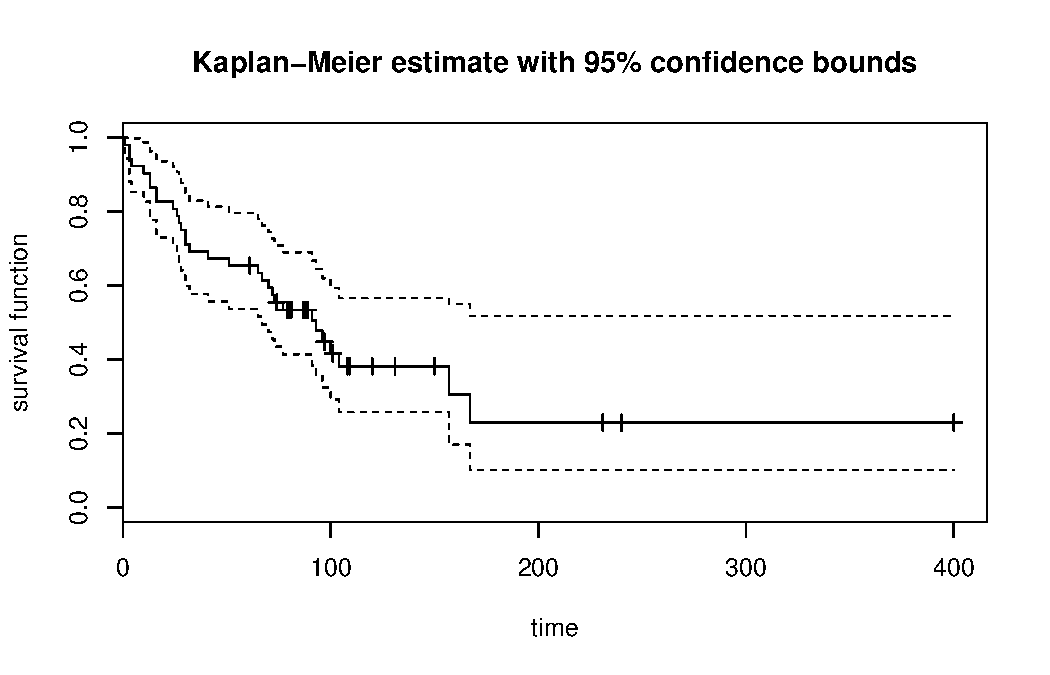
\includegraphics[height=2.8in]{../figures/kmPlot.pdf} \vspace{-4mm}
\caption{Sample output where only the title, x-axis and y-axis labels have been specified.}
\end{figure}
Sometimes different groups are mixed together in a single \rcom{Surv} object. If a separate vector containing a 'key' to which event times and censoring values correspond to which groups, then these groups can be separated by regressing the \rcom{Surv} object on the key:
\begin{verbatim}
> my.fit1 <- survfit( Surv(time, delta) ~ type )   # here the 'key' is 'type'
\end{verbatim}
The summary of \rcom{my.fit1} will contain an additional list item -- \rcom{strata}, accessible via \rcom{summary(my.fit1)\$strata} -- which designates which components of the output correspond to which groups.

Finally, for good coding practices, we detach the \rcom{tongue} data set.
\begin{verbatim}
> detach(tongue)
\end{verbatim}

%\textbf{Other options:} The \rcom{type} argument offers alternative estimates. The default is the Kaplan-Meier estimate (\rcom{'kaplan-meier'}) while other options are \rcom{'fleming-harrington'} and \rcom{'fh2'}. 


\pagebreak

%%% Confidence Bands %%%
\phantomsection
\tTitle{Confidence bands} \vspace{-1mm}\par
\tTitle{\rcom{conf.bands(x, conf.type='plain', type='ep', tL=NA, tU=NA)}}
\label{confBands}

The confidence intervals constructed on the previous pages are only pointwise confidence intervals. Confidence bands, which are a bit more generalized, can also be constructed. These bands provide bounds on an entire range of time. That is, for a 95\% confidence band, the probability that any part of the true curve is out of the confidence bands is 0.05. No functions within the package \package{survival} will create confidence bands. However, a custom function was written to fill this gap that can be downloaded:
\begin{verbatim}
> source('http://ddiez.com/teac/surv/conf-bands.R')
\end{verbatim}
A confidence ban is obtained by inputing a survival object for \rcom{x}. The \rcom{conf.type} may be \rcom{'plain'},  \texttt{'log-log'}, or \texttt{'asin-sqrt'}. The \texttt{type} argument may be \texttt{'ep'} or \texttt{'hall'} (Hall-Wellner). The \texttt{tL} and \texttt{tU} are optional to limit the scope of the confidence bands' meaning to hold from \texttt{tL} to \texttt{tU}. The appropriate value, $c_\alpha(a_L, a_U)$ for EP or $k_\alpha(a_L, a_U)$ for Hall-Wellner, must be input when requested by \texttt{conf.bands()}:
\begin{verbatim}
> data(bmt); attach(bmt)
> my.surv <- Surv(t2[group==1], d3[group==1])
> my.cb <- conf.bands(my.surv, type='hall', 100, 600)
   a_L: 0.1052632   |   a_U: 0.594237
   Enter confidence coefficent: 1.3211
> plot(survfit(my.surv), xlim=c(100, 600), xlab='time',
+   ylab='Estimated Survival Function', main='Reproducing 
+   Confidence Bands for Example 4.2 in Klein/Moeschberger')
\end{verbatim}
\begin{figure}[htp]
\centering
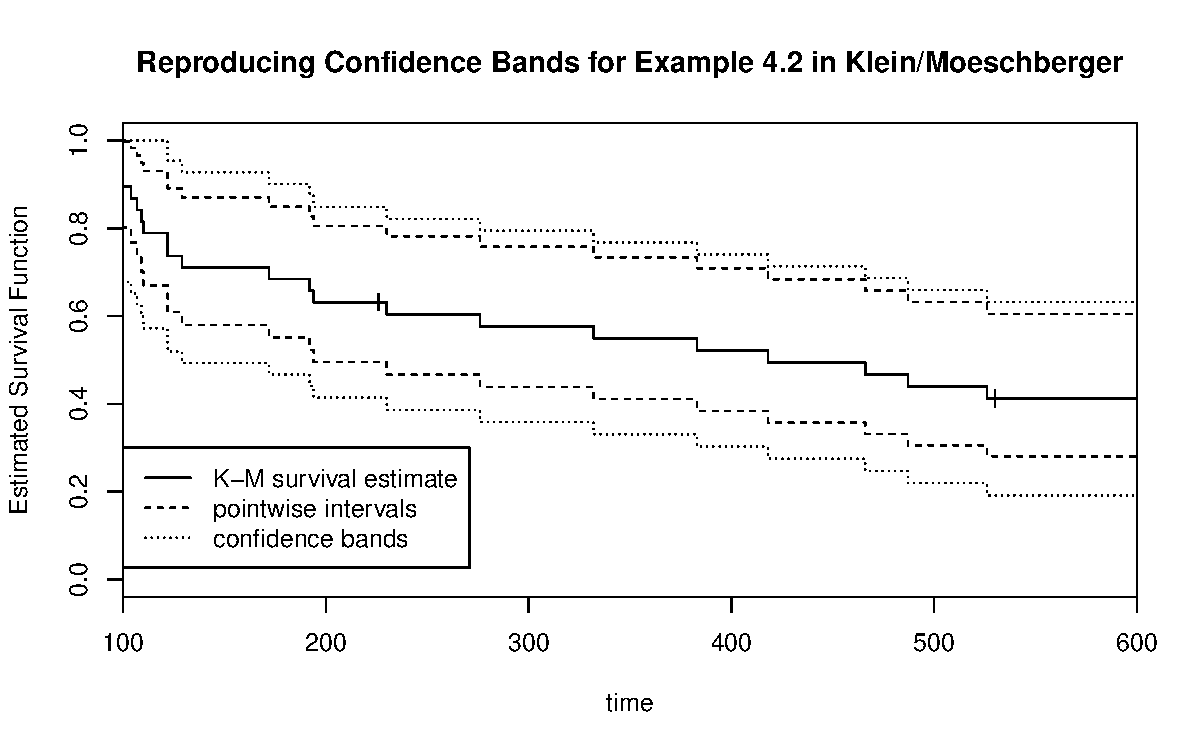
\includegraphics[height=2.3in]{../figures/confBand.pdf} \vspace{-4mm}
\caption{Confidence intervals and bans. The default for the pointwise confidence bands is a log transformation, which results in non-symmetric pointwise confidence intervals.}
\end{figure}
\begin{verbatim}
> lines(my.cb$time, my.cb$lower, lty=3, type='s')
> lines(my.cb$time, my.cb$upper, lty=3, type='s')
> legend(100, 0.3, legend=c('K-M survival estimate',
+   'pointwise intervals','confidence bands'), lty=1:3)
> detach(bmt)
\end{verbatim}

\pagebreak

%%% Cumulative Hazard %%%
\phantomsection
\tTitle{Cumulative Hazard}
\label{cumulativeHazard}

The cumulative hazard function and the survival function are related in the following way for continuous data:
\begin{align*}
S(t) = \exp\left\{-H(t)\right\}
\end{align*}
The MLE of the hazard function may be obtained by the inverse transformation of the Kaplan-Meier estimate: $\hat{H}(t) = -\log\hat{S}(t)$. Another method to estimate $H(t)$ is the Nelson-Aalen estimator:
\begin{align*}
\tilde{H}(t) &= \sum_{t_i \leq t} \frac{d_i}{Y_i}\text{ (assuming }t_1\leq t\text{, otherwise it is 0), }
		\qquad \sigma_H^2(t) = \sum_{t_i\leq t}\frac{d_i}{Y_i^2}
\end{align*}
No function in the \package{survival} package computes either form of the cumulative hazard function, but this can be accomplished using output from \texttt{survfit()}:
\begin{verbatim}
> data(tongue); attach(tongue)
> my.surv <- Surv(time[type==1], delta[type==1])
> my.fit  <- summary(survfit(my.surv ~ 1))
> H.hat   <- -log(my.fit$surv)
> H.hat   <- c(H.hat, tail(H.hat, 1))
\end{verbatim}
A summary plot or table may be created using \texttt{H.hat} with \texttt{my.fit\$time}. The Nelson-Aalen estimator may also be constructed:
\begin{verbatim}
> h.sort.of <- my.fit$n.event / my.fit$n.risk
> H.tilde   <- cumsum(h.sort.of)
> H.tilde   <- c(H.tilde, H.tilde[length(H.tilde)])
> plot(c(my.fit$time, 250), H.hat, xlab='time', ylab='cumulative hazard',
+   main='comparing cumulative hazards', ylim=range(c(H.hat, H.tilde)), type='s')
> points(c(my.fit$time, 250), H.tilde, lty=2, type='s')
> legend('topleft', legend=c("H.hat","H.tilde"), lty=1:2)
> detach(tongue)
\end{verbatim}
\begin{figure}[htp]
\centering
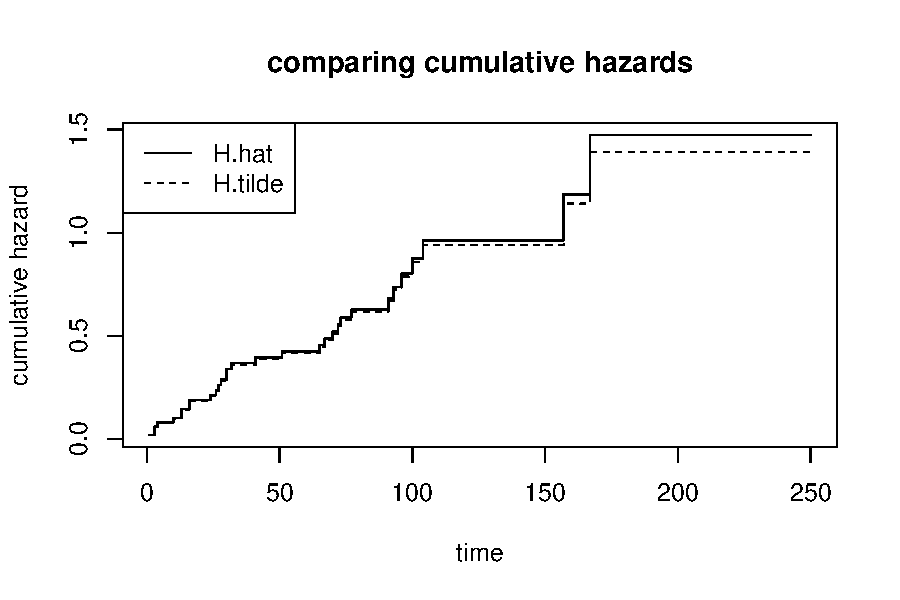
\includegraphics[height=2.5in]{../figures/cumHazard} \vspace{-4mm}
\caption{Cumulative hazard estimates.}
\end{figure}

\pagebreak

%%% Compute mean and median estimates %%%
\phantomsection
\tTitle{Mean and median estimates with bounds}
\label{meanAndMedianEstimates}

The median survival time is the time $t_{0.5}$ such that $S(t_{0.5}) = 0.5$. This is visualized by graphing the survival function estimate and drawing a horizontal line at 0.5. The median estimate equals the time $\hat{t}_{0.5}$ where the function and line intersect. The confidence bounds for $t_{0.5}$ are given by the points at which this horizontal line crosses over the confidence bounds of $\hat{S}(t)$.

\noindent The mean survival time and its respective estimate are given by
\begin{align*}
\mu &= \int_0^\infty S(t)dt, \qquad\hat{\mu} = \int_0^\infty \hat{S}(t)dt
\end{align*}
If $S(t)$ (or $\hat{S}(t)$) does not converge to zero, the integral diverges. One approach is to use a finite value $\tau$ as the bound for the integral. This results in a new statistic and corresponding estimate: $\mu_\tau = \int_0^\tau S(t)dt$. For instance, one might choose $\tau$ as the largest observed or censored time. Letting $t_i$, $Y_i$, $d_i$, and $D$ be as described in the Kaplan-Meier estimate, the estimated variance of $\hat{\mu}_\tau$ is
\begin{eqnarray*}
\hat{V}(\hat{\mu}_\tau) = \sum_{i=1}^D\left[\int_{t_i}^\tau \hat{S}(t)dt\right]^2 \frac{d_i}{Y_i(Y_i-d_i)}
\end{eqnarray*}

The median and its bounds may be estimated using \texttt{survfit()}:
\begin{verbatim}
> data(drug6mp); attach(drug6mp)
The following object(s) are masked from 'drug6mp (position 3)':

    pair, relapse, remstat, t1, t2
> my.surv <- Surv(t1, rep(1, 21))   # all placebo patients observed
> survfit(my.surv ~ 1)
Call: survfit(formula = my.surv ~ 1)

records   n.max n.start  events  median 0.95LCL 0.95UCL 
     21      21      21      21       8       4      12 
\end{verbatim}
Using \texttt{survfit()} in conjunction with \texttt{print()}, the mean survival time and its standard error may be obtained:
\begin{verbatim}
> print(survfit(my.surv ~ 1), print.rmean=TRUE)
Call: survfit(formula = my.surv ~ 1)

   records      n.max    n.start     events     *rmean *se(rmean) 
     21.00      21.00      21.00      21.00       8.67       1.38 
    median    0.95LCL    0.95UCL 
      8.00       4.00      12.00 
    * restricted mean with upper limit =  23 
> detach(drug6mp)
\end{verbatim}
The \texttt{print.rmean=TRUE} argument is used to obtain the mean and its standard error, and $\tau$ is automatically set as the largest observed or censored time. Alternatively, $\tau$ may be specified using the \texttt{rmean} argument.

\pagebreak

%%% Test difference of 2 survival curves %%%
\phantomsection
\tTitle{Tests for two or more samples} \vspace{-1mm}\par
\tTitle{\texttt{survdiff(formula, rho=0)}}
\label{testsForTwoOrMoreSamples}

Given two or more samples, is there a difference between the survival times? Setting up hypotheses for this problem,
\begin{itemize}
\item $H_0: h_1(t) = h_2(t) = \cdots = h_n(t)$ for all $t$.
\item $H_A: h_i(t_0)\neq h_j(t_0)$ for at least one pair $i,j$ and time $t_0$.
\end{itemize}
Let
\begin{itemize}
\item $t_{i}$ be times where events are observed (assume these are ordered and there are $D$ such times),
\item $d_{ik}$ be the number of observed events from group $k$ at time $t_i$,
\item $Y_{ik}$ be the number of subjects in group $k$ that are at risk at time $t_i$,
\item $d_{i} = \sum_{j=1}^n d_{ij}$,
\item $Y_{i} = \sum_{j=1}^n Y_{ij}$, and
\item $W(t_i)$ be the weight of the observations at time $t_i$.
\end{itemize}
Then to test the hypothesis above, a vector $Z$ is computed, where
\begin{eqnarray*}
Z_k = \sum_{i=1}^D W(t_i)\left[d_{ik} - Y_{ik}\frac{d_{i}}{Y_{i}}\right]
\end{eqnarray*}
The covariance matrix $\widehat{\Sigma}$ is also computed from the data (see \refBib{Klein2003}). Under the null hypothesis, the test statistic $X^2 = Z'\hat{\Sigma}^{-1}Z$ follows a $\chi^2$ distribution with $n$ degrees of freedom. That is, if $X^2 > \chi^2_{1-\alpha, df=n}$, the data provides convincing evidence against null hypothesis (we reject $H_0$).

The function \texttt{survdiff()} is used for this hypothesis test. The first argument is a survival object against a categorical covariate variable that is typically a variable designating which groups correspond to which survival times. The output directly from \texttt{survdiff()} is of most use (\texttt{summary()} of a \texttt{survdiff()} object does not provide much information).
\begin{verbatim}
> data(btrial); attach(btrial)       # time variable warning omitted
> survdiff(Surv(time, death) ~ im)   # output omitted
\end{verbatim}
The second argument shown, \texttt{rho}, designates the weights according to $\hat{S}(t)^\rho$ and may be any numeric value. The default is \texttt{rho=0} and corresponds to the log-rank test. The \term{Peto \& Peto modification of the Gehan-Wilcoxon test} is computed using \texttt{rho=1}:
\begin{verbatim}
> survdiff(Surv(time, death) ~ im, rho=1)   # some output omitted
...

 Chisq= 4.4  on 1 degrees of freedom, p= 0.037 
> detach(btrial)
\end{verbatim}
To give greater weight to the first part of the survival curves, use \texttt{rho} larger than \texttt{0}. To give weight to the later part of the survival curves, use \texttt{rho} smaller than \texttt{0}. The output of \texttt{survdiff()} is generally self-explanatory. A $\chi^2$ statistic is computed along with a p-value.

\pagebreak

%%% Cox PH Models %%%
\phantomsection
\tTitle{Cox proportional hazards model, constant covariates} \vspace{-1mm} \par
\tTitle{\texttt{coxph(formula, method)}}
\label{coxPHConstCov}

The Cox PH model fits survival data with covariates $z$ to a hazard function of the form
\begin{eqnarray*}
h(t|z) = h_0(t)\exp\left\{ \beta'z  \right\}
\end{eqnarray*}
where $\beta$ is an unknown vector. $h_0(t)$ is the \textit{baseline hazard}, which is non-parametric. Primary interest lies in finding the parameter $\beta$, which is found by solving the partial likelihood:
\begin{eqnarray*}
L(\beta) = \prod_{i=1}^D \frac{\exp\left[\beta'z_{(i)}\right]}{\sum_{j \in R(t_i)}\exp\left\{\beta'z_j\right\}}, \text{ }R(t_i)\text{ is the 'risk set' at time }t_i
\end{eqnarray*}
The MLE $\hat{\beta}$ (a vector) is asymptotically $N(\beta, I^{-1})$, where $I$ represents the covariance matrix of $\beta$ (typically estimated). This normal approximation makes doing local tests possible. A \term{local test} examines a subset of the elements of $\beta$, testing the claim $C\beta = d$, where $C$ is a $q\times p$ matrix of full rank and $d$ is a vector of length $q$. Under this setup, the test statistic is
\begin{eqnarray*}
X_W^2 = \left(C\hat{\beta} - d\right)'\left[C\hat{I}^{-1}C'\right]^{-1}\left(C\hat{\beta} - d\right),
\end{eqnarray*}
which under the null hypothesis follows $\chi^2_q$. This is known as the \term{Wald test}.

Beyond obtaining test p-values, there may be interest in the survival function for particular covariates. If the estimate of the baseline survival function, $\hat{S}_0(t)$, is provided, then the estimate of the survival function for an individual with covariates $z_k$ may be obtained via
\begin{eqnarray*}
\hat{S}(t|z_k) = \left[\hat{S}_0(t)\right]^{\exp\left(\hat{\beta}'z_k \right)}
\end{eqnarray*} 

The function \rcom{coxph()} fits a Cox PH model to the supplied data. The first argument is a formula, where the response is a survival object. %The second argument, \rcom{method}.
\begin{verbatim}
> data(burn); attach(burn)
> my.surv <- Surv(T1, D1)
> coxph(my.surv ~ Z1 + as.factor(Z11), method='breslow')
Call:
coxph(formula = my.surv ~ Z1 + as.factor(Z11), method = "breslow")


                  coef exp(coef) se(coef)     z     p
Z1               0.497     1.644    0.208  2.38 0.017
as.factor(Z11)2 -0.877     0.416    0.498 -1.76 0.078
as.factor(Z11)3 -1.650     0.192    0.802 -2.06 0.040
as.factor(Z11)4 -0.407     0.666    0.395 -1.03 0.300

Likelihood ratio test=14.6  on 4 df, p=0.00569  n= 154 
\end{verbatim}
Two covariates have been used in this example. The second argument listed, \rcom{method}, specifies how ties are handled. The default is \rcom{'efron'}, and the other options are \rcom{'breslow'} and \rcom{'exact'}. Much useful information is obtained in the summary of \rcom{coxph()}, including
\begin{itemize}
\item estimates of the $\beta_k$, including standard errors and p-values for each test $H_0: \beta_k=0$, % with the other $\beta_j = \hat{\beta}_j$,
\item estimate of the risk ratio with confidence bounds, and
\item p-values for likelihood ratio, Wald and score tests for the global null, $H_0: \beta_i =0$ for all $i$.
\end{itemize}
More complex hypotheses may be checked using other output from the model fit:
\begin{verbatim}
> coxph.fit <- coxph(my.surv ~ Z1 + as.factor(Z11), method='breslow')
> coxph.fit$coefficients  # may use my.fit$coeff instead
> coxph.fit$var           # I^(-1), estimated cov matrix of the beta-hats
> coxph.fit$loglik        # log-likelihood for alt and null MLEs, resp.
\end{verbatim}
To obtain the baseline survival function from a Cox PH model, apply \rcom{survfit()} to \rcom{coxph()}:
\begin{verbatim}
> my.survfit.object <- survfit(coxph.fit)
\end{verbatim}
The output from \rcom{survfit()} are all the same as when it was applied to a survival object (and it may be plotted, just like the previous \rcom{survfit()} objects).

A rudimentary function for doing local checks when $C$ and $d$ may be loaded via
\begin{verbatim}
> source('http://ddiez.com/teac/surv/local-coxph-test.R')
\end{verbatim}
The function loaded is called \rcom{local.coxph.test} and its format is
\begin{verbatim}
    local.coxph.test(coxph.fit, pos, C=NA, b=NA)
\end{verbatim}
The first argument is an output from \rcom{coxph()}, \rcom{pos} is a vector of describing which betas to include in the test (e.g. \rcom{pos=c(2,4)} for the second and fourth betas), and \rcom{C} and \rcom{d} are matrices describing the null. This function is especially helpful in determining whether a factor variable should be included in a model:
\begin{verbatim}
> coxph.fit
...
                  coef exp(coef) se(coef)     z     p
Z1               0.497     1.644    0.208  2.38 0.017
as.factor(Z11)2 -0.877     0.416    0.498 -1.76 0.078
as.factor(Z11)3 -1.650     0.192    0.802 -2.06 0.040
as.factor(Z11)4 -0.407     0.666    0.395 -1.03 0.300
...
> local.coxph.test(coxph.fit, 2:4)
[1] 0.103
> detach(burn)
\end{verbatim}
In this example, \rcom{Z11} was a factor variable estimated in the second, third, and fourth coefficients from \rcom{my.fit}. The p-value of the test was 0.103, i.e. \rcom{Z11} is not statistically significant for $\alpha=0.05$.

A more thorough look at Cox PH models beyond what is discussed here is available in \refBib{Fox2002}.

\pagebreak

%%% Cox PH time-dependent Models %%%
\phantomsection
\tTitle{Cox proportional hazards model, time-dependent covariates}
\label{coxPHTimeDepCov}

Using time-dependent covariates in R is an exercise in organization. Previously considered covariates were unchanging attributes, such as treatment group or control group or a patient's race. Now we consider time-dependent covariates, such as interventions or environmental factors that change.

To use time-dependent covariates in R, we use left-truncation liberally. For example, if there is an intervention for patient $i$, then we split patient $i$ into two separate observations: pre and post-intervention. More explicitly, suppose the patient intervention took place at time $t_{i} = 45$ and the event for patient $i$ was observed at $t_{event}=58$. Then in R, we would split this patient's record into two pieces: 0 to 45 and 45 to 150. We can assign the covariate for intervention differently for each interval. In applying this method in R, we must be careful to provide start and end times for each interval and also indicate censoring.

We consider the following example (simulated data). Patients records from one rehabilitation clinic were obtained for 150 days after they became sober. The event of interest was drug-relapse and two covariates were recorded. The \rcom{time} variable describes the observed or censored time; the \rcom{event} variable describes whether the time denotes an observed relapse (\rcom{TRUE}) or a censored time; the \rcom{gender} variable is a time-independent covariate; and \rcom{int} is a time-depedent covariate indicating whether the patient had an intervention. All interventions occurred \emph{after} the patients became sober (day 0), meaning the intervention covariate changes over time for those patients who had an intervention before relapse. % Not all patients had interventions before relapsing or the end of the study.
\begin{verbatim}
> relapse
    time event gender int
1    150 FALSE      0  84
2     53  TRUE      1  50
3     12  TRUE      1  NA
4    150 FALSE      0  89
5    150 FALSE      1  77
...
299   10  TRUE      0  NA
300   94  TRUE      1   4
\end{verbatim}

To model this data within R, we proceed in two steps:
\begin{enumerate}
\item Construct survival records that may include left and right-censored observations. The survival record of each patient with an intervention is broken into two survival records: one before the intervention and one after. This step is largely book-keeping and programming in R.
\item The new survival records can be run through the \rcom{coxph()} function.
\end{enumerate}
We begin with the construction of proper survival records.
%\textbf{Construction of proper survival records.} \par
%\begin{itemize}
%\item[] 
We first initialize new values for each input parameter for the survival records to be input into \rcom{Surv()}.
% a patient never had the new intervention before relapsing, she has no covariates that change over time. That is, we need not adjust her representation in the data. If a patient did have an intervention, then we would like to model how this intervention impacted the patient. Patients who had an intervention prior to relapsing have a time-changing covariate, and to incorporate the covariate, their observations are split into a ``new'' patient whenever that covariate changes. For the example, the new variables are first initialized:
%Then each patient is examined. Records of patients with no intervention are simply maintained. The records of patients who had an intervention will be split into two pieces: pre and post-intervention.
\begin{verbatim}
> N  <- dim(relapse)[1]
> t1 <- rep(0, N+sum(!is.na(relapse$int)))  # Initialize start time at 0
> t2 <- rep(-1, length(t1))                 # Build vector for end times
> e  <- rep(-1, length(t1))                 # Whether event was censored
> g  <- rep(-1, length(t1))                 # Gender covariate
> i  <- rep(FALSE, length(t1))              # Initialize intervention at FALSE
\end{verbatim}
Next, each patient is checked for whether they had an intervention. If they did not, then their record is simply copied to the new variables used. If there was an intervention, their observations are split into two pieces: the period prior to intervention and the period after intervention. The period after intervention is left-truncated.
\begin{verbatim}
> j  <- 1
> for(ii in 1:dim(relapse)[1]){
+   if(is.na(relapse$int[ii])){      # no intervention, copy survival record
+     t2[j] <- relapse$time[ii]
+     e[j]  <- relapse$event[ii]
+     g[j]  <- relapse$gender[ii]
+     j <- j+1
+   } else {                         # intervention, split records
+     g[j+0:1] <- relapse$gender[ii] # gender is same for each time
+     e[j]     <- 0                  # no relapse observed pre-intervention
+     e[j+1]   <- relapse$event[ii]  # relapse occur post-intervention?
+     i[j+1]   <- TRUE               # Intervention covariate, post-intervention
+     t2[j]    <- relapse$int[ii]-1  # End of pre-intervention
+     t1[j+1]  <- relapse$int[ii]-1  # Start of post-intervention
+     t2[j+1]  <- relapse$time[ii]   # End of post-intervention
+     j <- j+2                       # Two records added
+   }
+ }
\end{verbatim}
Now we have a number of new variables. The \rcom{t1} variable represents the start of each interval; \rcom{t2} the end of each interval; \rcom{e} indicates if the event -- the relapse -- was observed; \rcom{g} is the gender covariate; and \rcom{i} is the indicator variable for whether this interval is associated with a patient post-intervention.

While each patient was permitted to have time-varying covariates, each of the new intervals has covariates that do not change, so the survival object and Cox PH model can be constructed:
\begin{verbatim}
> mySurv <- Surv(t1, t2, e)
> myCPH  <- coxph(mySurv ~ g + i)
\end{verbatim}

This example was a simple case: there was a single time-dependent covariate, and it changed at most once per case. In some instances, there may be many time-varying covariates, even some that change every time unit. In most of these instances, the same method may be used. Whenever a covariate changes from one time unit to the next, split the interval into two and use censoring.

For additional reading on time-dependent covariates in R, see pages 7-11 of \refBib{Fox2002}.

%One case of interest is creating a new time-dependent covariate, $Z_i^t$, from another covariate, $Z_i$. This may be done by using a transformation on the time and multiply the result by $Z_i$:
%\begin{eqnarray*}
%Z_i^t = Z_i * transformation(t)
%\end{eqnarray*}
%A common transformation is $\log$ but others may be used. A function to create a type of variable of this form and also to run a Cox PH model with it is the following:
%\begin{verbatim}
%timeDepCoxph(x, colTime, colDelta, colCov, tdCov, transform=log,
%   outputModel=TRUE, outputDF=FALSE, verbose=TRUE, ...)
%\end{verbatim}
%The function is included in the \package{OIsurv} package. Here,
%\begin{itemize}
%\item \rcom{x} is a data frame with all of the original data,
%\item \rcom{colTime} is the name/number indicating which column of \rcom{x} is the event/right-censored time,
%\item \rcom{colDelta} is the name/number representing the column of \rcom{x} indicates observed events,
%\item \rcom{colCov} is a vector of the column numbers/names of the covariates to be included in the model, and
%\item \rcom{tdCov} is the column number/name of the covariate $Z_i$ to be used to create the time-dependent covariate. $Z_i$ must be a vector with only 2 unique numerical values. (e.g. $Z_i$ is a vector of \rcom{0}'s and \rcom{1}'s).
%\end{itemize}
%The following arguments have defaults, as are specified above:
%\begin{itemize}
%\item \rcom{transform} is the type of transformation to be used on time,
%\item \rcom{outputModel} indicates whether the Cox PH model should be included in the output,
%\item \rcom{outputDF} indicates whether the time-dependent data frame that was created should be output (this may be useful if many closely related models are going to be checked), and
%\item \rcom{verbose} indicates whether the user should be notified at how far along the function is at computing the data frame to be used in the Cox PH model (this is useful to see how fast the function is running).
%\item Additional arguments are passed to \rcom{coxph()},
%\end{itemize}
%Below is an example of how to use this function:
%\begin{verbatim}
%> data(burn)
%> attach(burn)
%> td.coxph <- timeDepCoxph(burn, 'T1', 'D1', 2:4, 'Z1', verbose=FALSE)
%\end{verbatim}
%The covariates in the output will be of the same order as specified in \rcom{colCov}.
%\begin{verbatim}
%> td.coxph   # some model output is omitted for brevity
%...
%                coef exp(coef) se(coef)      z      p
%Z1            1.3569     3.884    0.719  1.886 0.0590
%Z2            0.6899     1.994    0.231  2.981 0.0029
%Z3            0.0496     1.051    0.302  0.164 0.8700
%time.dep.cov -0.3383     0.713    0.312 -1.085 0.2800
%\end{verbatim}
%The default output of \rcom{timeDepCoxph()} is the output of \rcom{coxph()}. It has all the usual outputs of \rcom{coxph()}. For example, log-likelihood:
%\begin{verbatim}
%> td.coxph$loglik
%[1] -420.4825 -411.8814
%> detach(burn)
%\end{verbatim}

\pagebreak




% - - - - - AFT models  - - - - - %
\phantomsection
\tTitle{Accelerated failure-time models} \vspace{-1mm} \par
\tTitle{\rcom{survreg(formula, dist='weibull')}}
\label{accFailureTimeModels}

An accelerated failure-time (AFT) model is a parametric model with covariates and failure times follow the survival function $S(x|Z) = S_0\left(x*\exp\left[ \theta'Z \right]\right)$, where $S_0$ is a function for the baseline survival rate. The term $\exp\left[\theta'Z\right]$ is called the \term{acceleration factor}. The AFT model uses covariates to place individuals on different time scales -- note the scaling by the covariates in $S(t|Z)$ via $\exp\left[ \theta'Z \right]$. The AFT model can be rewritten to a log-linear form, where the log of failure time $\log X$ is linearly related to the mean $\mu$, the acceleration factor, and an error term $\sigma W$:
\begin{eqnarray*}
\log X = \mu - \theta'Z + \sigma W
\end{eqnarray*}
%The main choice to be made is which distribution to use for the error. The options discussed in Klein and Moeschberger are shown in the table below:
where $W$ describes the error distribution. The following models for $W$ are discussed in \refBib{Klein2003}:
\begin{quotation}\center
\begin{tabular}{llcc}
\hline 
\hline
distribution & \rcom{  } & df & included in \package{survival}? \\
\hline 
exponential & & 1 & yes \\
Weibull & & 2 & yes \\
lognormal & & 2 & yes \\
log logistic & & 2 & yes \\
generalized gamma & & 3 & no \\
\hline
\hline
\end{tabular}
\end{quotation}

The function \rcom{survreg()} function from the \package{survival} package is used for AFT modeling. The first argument is \rcom{formula} or a survival object regressed on predictors. The argument \rcom{dist} has several options to describe the parametric model used (\rcom{'weibull'}, \rcom{'exponential'}, \rcom{'gaussian'}, \rcom{'logistic'}, \rcom{'lognormal'}, and \rcom{'loglogistic'}). The example code below follows Example 12.2 from \refBib{Klein2003}:
\begin{verbatim}
> data(larynx)
> attach(larynx)
> srFit <- survreg(Surv(time, delta) ~ as.factor(stage) + age, dist='weibull')
> summary(srFit)
...
                    Value Std. Error      z        p
(Intercept)        3.5288     0.9041  3.903 9.50e-05
as.factor(stage)2 -0.1477     0.4076 -0.362 7.17e-01
as.factor(stage)3 -0.5866     0.3199 -1.833 6.68e-02
as.factor(stage)4 -1.5441     0.3633 -4.251 2.13e-05
age               -0.0175     0.0128 -1.367 1.72e-01
Log(scale)        -0.1223     0.1225 -0.999 3.18e-01

Scale= 0.885 

Weibull distribution
Loglik(model)= -141.4   Loglik(intercept only)= -151.1
	Chisq= 19.37 on 4 degrees of freedom, p= 0.00066 
Number of Newton-Raphson Iterations: 5 
...
\end{verbatim}
In the output, \rcom{(Intercept)} and \rcom{Log(scale)} correspond to estimates of $\mu$ and $\log\sigma$. The other estimates correspond to covariate coefficients. %Models may be comparatively assessed using the AIC:
%\begin{eqnarray*}
%AIC = -2\log L + 2p
%\end{eqnarray*}
%where $L$ is the likelihood. In this case, the AIC is equal to 294.8 ($p=6$). %The AIC may be used for model selection (fit several models and determine which has the lowest AIC). For example, we may fit an exponential model on the same data to find the AIC of this model and compare:
We might compare this to a result for the exponential model, where the scale is fixed at 1:
\begin{verbatim}
> srFitExp <- survreg(Surv(time, delta) ~ as.factor(stage) + age, dist='exponential')
> summary(srFitExp)
...
                    Value Std. Error      z        p
(Intercept)        3.7550     0.9902  3.792 1.49e-04
as.factor(stage)2 -0.1456     0.4602 -0.316 7.52e-01
as.factor(stage)3 -0.6483     0.3552 -1.825 6.80e-02
as.factor(stage)4 -1.6350     0.3985 -4.103 4.08e-05
age               -0.0197     0.0142 -1.388 1.65e-01

Scale fixed at 1 

Exponential distribution
Loglik(model)= -141.9   Loglik(intercept only)= -151.1
	Chisq= 18.44 on 4 degrees of freedom, p= 0.001 
Number of Newton-Raphson Iterations: 4 
...
\end{verbatim}
%The AIC for the exponential is 293.8 ($p=5$). Because the $293.8 < 294.8$, the AIC suggests the exponential model may be more appropriate.

The Weibull model with $\sigma=1$ is equivalent to the exponential model. We consider two strategies for selecting which of the two models is more appropriate:
\begin{itemize}
\item A likelihood ratio test, which evaluates the null hypothesis $\sigma=1$ against the two-sided alternative.
\item Examination of the significance of the \rcom{Log(scale)} coefficient (see the output to \rcom{summary(srFit)}).
\end{itemize}
In the example, both approaches result in the same conclusion: there is insufficient evidence to reject the notion that $\sigma=1$ ($H_0$).

Interested users may explore the many stored components in a \rcom{survreg()} object:
\begin{verbatim}
> # the output is omitted from each command below
> srFitExp$coeff    # covariate coefficients
> srFitExp$icoef    # intercept and scale coefficients
> srFitExp$var      # variance-covariance matrix
> srFitExp$loglik   # log-likelihood
> srFit$scale       # not using srFitExp (defaulted to 1)
> detach(larynx)
\end{verbatim}

\pagebreak

%\tTitle{Acknowledgements}

%\vspace{4mm}

%Thank you to Gang Li, who taught me everything I know about survival analysis and encouraged me to write this guide for my course project.

%\vspace{15mm}

\phantomsection
\tTitle{References}
\label{references}

\vspace{4mm}

\bibItem{R}{R Development Core Team (2010). R: A language and environment for statistical computing. R Foundation for Statistical Computing, Vienna, Austria. ISBN 3-900051-07-0, URL \url{http://www.R-project.org.}}

\bibItem{survivalPackage}{Terry Therneau and original R port by Thomas Lumley (2009). survival: Survival analysis, including penalised likelihood. R package version 2.35-8. \vspace{-2mm}\par \url{http://CRAN.R-project.org/package=survival}.}

\bibItem{KMsurvPackage}{Original by Klein, Moeschberger and modifications by Jun Yan (2010). KMsurv: Data sets from Klein and Moeschberger (1997), Survival Analysis. R package version 0.1-4. \vspace{-2mm}\par \url{http://CRAN.R-project.org/package=KMsurv}.}

\bibItem{Klein2003}{Klein, John P., and Melvin L. Moeschberger. Survival Analysis: Techniques for Censored and Truncated Data. New York: Springer, 2003.}

\bibItem{formsOfSurvData}{ReliaSoft Corporation website (2006). Data Classification. \vspace{-2mm}\par \url{http://www.weibull.com/LifeDataWeb/data_classification.htm}}.

\bibItem{Fox2002}{Fox, John 2002. Cox Proportional-Hazards Regression for Survival Data. Appendix to An R and S-PLUS Companion to Applied Regression.}

\vspace{15mm}

\tTitle{Additional resources}

\vspace{4mm}

\bibItem{Lumley2007}{Lumley, Thomas, 2007. The Survival Package (R help guide).}






\end{document}   